% easychair.tex,v 3.4 2015/12/10

\documentclass{easychair}
%\documentclass[EPiC]{easychair}
%\documentclass[debug]{easychair}
%\documentclass[verbose]{easychair}
%\documentclass[notimes]{easychair}
%\documentclass[withtimes]{easychair}
%\documentclass[a4paper]{easychair}
%\documentclass[letterpaper]{easychair}
\newcommand{\specialcell}[2][c]{%
  \begin{tabular}[#1]{@{}c@{}}#2\end{tabular}}

\usepackage{doc}

%use packages added by karla
\usepackage[utf8]{inputenc}
\usepackage[english]{babel}
\usepackage{color}
%use packages added by karla

%use packages added by Colin
 \usepackage{multirow}
 \usepackage{graphicx}
 %use packages added by Colin

% use this if you have a long article and want to create an index
% \usepackage{makeidx}

% In order to save space or manage large tables or figures in a
% landcape-like text, you can use the rotating and pdflscape
% packages. Uncomment the desired from the below.
%
% \usepackage{rotating}
% \usepackage{pdflscape}

% Some of our commands for this guide.
%
\newcommand{\easychair}{\textsf{easychair}}
\newcommand{\miktex}{MiK{\TeX}}
\newcommand{\texniccenter}{{\TeX}nicCenter}
\newcommand{\makefile}{\texttt{Makefile}}
\newcommand{\latexeditor}{LEd}

%\makeindex

%% Front Matter
%%
% Regular title as in the article class.
%
% \title{The {\easychair} Class File\\
%        Documentation and Guide for Authors%
% \thanks{Other people who contributed to this document include Maria Voronkov
%   (Imperial College and EasyChair) and Graham Gough (The University of
%   Manchester).}}

% \title{Reconciling SCXML and Event-B Semantics}
% \title{Generating Event-B from a Statechart Representation}
% \title{The use of SCXML to bridge Event-B and Higher level represetations}
\title{Reconciling SCXML Statechart Representations and Event-B Lower Level Semantics}
% \title{Statechart representation based on SCXML}

% Authors are joined by \and. Their affiliations are given by \inst, which indexes
% into the list defined using \institute
%
% \author{
% Serguei A. Mokhov\inst{1}\thanks{Designed and implemented the class style}
% \and
%     Geoff Sutcliffe\inst{2}\thanks{Did numerous tests and provided a lot of suggestions}
% \and
%    Andrei Voronkov\inst{3}\inst{4}\inst{5}\thanks{Masterminded EasyChair and created versions
%      3.0--3.4 of the class style}
% }

\author{
Karla Morris\inst{1}
\and
Colin Snook\inst{2}
}

% Institutes for affiliations are also joined by \and,
\institute{
  Sandia National Laboratories, 
  Livermore, California, U.S.A.\\
  \email{knmorri@sandia.gov}
\and
   University of Southampton,
   Southampton, United Kingdom\\
   \email{cfs@ecs.soton.ac.uk}\\
 }

%  \authorrunning{} has to be set for the shorter version of the authors' names;
% otherwise a warning will be rendered in the running heads. When processed by
% EasyChair, this command is mandatory: a document without \authorrunning
% will be rejected by EasyChair

\authorrunning{}

% \titlerunning{} has to be set to either the main title or its shorter
% version for the running heads. When processed by
% EasyChair, this command is mandatory: a document without \titlerunning
% will be rejected by EasyChair

\titlerunning{}

\begin{document}

\maketitle

\begin{abstract}
  BLA BLA 
\end{abstract}

% The table of contents below is added for your convenience. Please do not use
% the table of contents if you are preparing your paper for publication in the
% EPiC series

% \setcounter{tocdepth}{2}
% {\small
% \tableofcontents}

%\section{To mention}
%
%Processing in EasyChair - number of pages.
%
%Examples of how EasyChair processes papers. Caveats (replacement of EC
%class, errors).

\pagestyle{empty}

%------------------------------------------------------------------------------
\section{Introduction}
\label{sect:introduction}


% \begin{figure}[tb]
% 	\begin{centering}
% 	
\includegraphics[width=0.5\textwidth]{logoEC}
% 	\caption{EasyChair logo}
% 	\label{fig:easychair-logo}
% 	\end{centering}
% \end{figure}

% \textcolor{red}{This section should focus on the motivation behind pursuing a scxml 
% representation of our models, what are the benefits?}

The formal verification of high consequence systems 
requires the analysis of formal models that capture 
the properties and functionality of the system of 
interest. Discharging proof obligations for systems' 
properties or requirements can be made more tracktable 
depending on the abstraction use to create the model, 
as properties are expressed in term of variables that 
are relevant at different abstraction levels.  

A herarchical development of a system model makes 
use of refinement concepts to link the different levels
of abstraction. Each subsequent level increases model 
complexity by adding implementation details to the 
model in the form of functionality, capabilities and 
finner requirements. As the model complexity increases 
in each refinement level tractability of the model 
can be improve by the use of a graphical representation, 
with rich semantics that can support an infrastructure 
for formal verification.

The Event-B language provides the logic, and refinement
theory require to formaly analyze a system model. The 
open-source Rodin tool auments the Event-B language by 
providing a graphical interphace in the form of
iUML-B. The goal of this work is to create a unified model 
representation capable of leveraging the structure and 
herarchy that is inherently part of a statechart 
diagram, which will serve to enable the formal verification
of requirements from two different  perspective. First, 
the translation of the unified representation to Event-B. Second,
the analysis of requirements related to the structure of 
the statechart it self, which is a higher level representation 
of the model. 

We base this unified statechart model representaiton 
on SCXML.  This is a general-purpose event-based state machine 
language that combines concepts from CCXML and Harel 
State Tables. Harel State Tables are included in UML. 
The concrete syntax for SCXML\footnote{http://www.w3.org/TR/scxml/} 
is based on XML. Hence, SCXML is an XML notation for 
UML style state-machines extended with an action 
language that is intended for call control features 
in voice applications.

%------------------------------------------------------------------------------

\section{Reconciling SCXML and iUML-B Semantics}
\label{sect:recon}

The SCXML basic structure of states with nested 
statemachines and transitions is the same as that 
in iUML-B, but there are several semantic 
differences that make translation into iUML-B difficult. 
This sections provides a description of some of the
main differences, as well as possible solutions for their
reconciliation.

\begin{description}
\item [Refinement:]
Refinement is a central concept in iUML-B, detail is 
added in refinements by progressive hierarchical 
nesting. There is no refinement in SCXML. Features
in the diagrams have to be restricted to guarantee
that the models are correct refinements. An example,
of such a restriction is not allowing for actions in 
both parent and nested states to change the same varaible.

\item [Events:]
The meaning of event is very different between iUML-B 
and SCXML. In iUML-B transitions are sub-parts of 
events. In order for an event to be enabled for firing, 
all of its sub-parts (transitions) must be 
simultaneously enabled. This means that two different 
transitions with the same event can only fire at the 
same time and hence will never fire if they are sourced 
from different states of the same parent state-machine. 
In SCXML, events are triggers that enable transitions 
to fire. If two different transitions from different 
source states are both triggered by the same event, one 
may fire without the other if one source state is not 
active.

\item [Entry and Exit Actions:]
SCXML includes the concept of entry and exit actions 
which are executed whenever a transition enters and 
exits respectively, the containing state. 
iUML-B has been extended to support the construction 
of entry/exit actions.

The addition of these feature is straight forward,
however, the lack of sequential composition in 
Event-B (hence iUML-B) means that the semantics of entry/
exit actions will differ in some scenarios. That is, in 
SCXML the source state’s exit actions are taken before the 
transition’s actions, which are before the target state’s 
entry actions. In iUML-B all the actions are taken in 
parallel, as there is no concept of execution order within 
an event. 

We restrict SCXML so that the actions are parallelisable. 
Effectively this means that the same variable cannot be 
assigned more than once in any set of actions that will be 
taken when a transition fires. The Event-B static checker 
would then raise an error if the same variable is assigned 
in for example, the source states exit actions and the 
target states entry actions. 

% One difficulty arises when a transition exits a parent 
% state without specifying a particular nested sub-state. 
% Strictly, only the exit actions of the currently active sub-
% state should be executed. However, this would be difficult 
% in iUML-B due to the lack of any conditional execution.


\item [Transition firing:]
The hierarchical state constructs of both SCXML and
iUML-B are equivalent, but their transition 
firing mechanism differs significantly. In iUML-B 
transitions fire spontaneously when their guard and source 
state are true. In SCXML, there are two kinds of transitions, 
‘When’ transitions can fire spontaneously as soon as their 
guard becomes true. This is the same as iUML-B transitions 
and we have no problem translating these. Other SCXML
transitions are triggered by the 
occurrence of some other event, which may be external 
or internal (induced by the actions of another transition). 
In iUML-B if several transitions are simultaneously 
enabled one of the enabled transitions is non-deterministically 
chosen for firing whereas SCXML has ordering rules to 
determine which transitions to fire next.

Thigger events could be simulated by generating a flag to 
represent the trigger and adding a guard on the trigger 
flag to the transitions that are triggered by it. The flag 
should then be reset by whichever transition is triggered 
by it in order to ‘consume’ that trigger event. A special 
interface event that sets the flag would be generated to 
represent the external interface receiving a trigger.

Transitions may also trigger each other. This could be 
modelled by a similar mechanism except that the interface 
event is not needed since the flag is set directly by 
another transition.

% \item [Transition execution:]
% When a particular SCXML transition fires it carries out 
% a sequence of actions in particular order. For example, 
% a hierarchy of nested source states exit,
% performing exit actions starting from the innermost 
% one and working outwards. The order of the actions 
% is significant in SCXML as these actions could 
% write to the same variable. In Event-B all actions of a 
% transition are executed simultaneouslly within the elaborated 
% event. It is not possible (i.e. not well-formed) for two of these 
% actions to write to the same variable.
% SCXML transitions can be designated ‘internal’, which 
% prevents exiting and re-entering its source state in 
% some cases. In SCXML target state can be omitted which 
% results in a transition that does not change state (
% this is different from a transition that exits a state 
% and then re-enters the same state).
% Neither of these features is supported in iUML-B since 

\item [Run to completion semantics:] SCXML has a run-to-completion 
(or big-step/little-step) semantics. This means that an external 
trigger is only consumed when no transition can be taken without 
doing so. This is quite cumbersome to implement in iUML-B since 
it requires constructing the conjunction of the negated guards of
all the transitions that are internally triggered (including when 
transitions) and adding this to all externally triggered transitions.

\item [Final States:]
The concept of a final state differs between iUML-B and 
SCXML. In SCXML a state machine (or parent state) may 
reside in a final state indicating that it is done and 
waiting for another transition to exit the parent 
state.  In iUML-B a final state is not a proper state 
of the parent state-machine. It is merely a notation 
for indicating that the state-machine is becoming non-
active. I.e. that the parent state is exiting. Hence 
any transitions that target a final state are part of a 
transition that leaves the parent state. For a ‘root’ 
state-machine the final state means that the state-
machine has been left completely and no state is active.

\item [Initial States:]
Initial states are similar to iUML-B. The transition 
from the initial state forms part of the actions to 
enter the parent state. However, the correspondence 
between incoming transitions to the parent state and 
initial transitions is more explicit in iUML-B. 
SCXML has another way to specify an initial state using 
an attribute of the state. In this case there is no way 
to add extra transition actions.
If no initial state is specified, the default is the 
first one in the document.
iUML-B allows different intial states for different 
incoming transitions. In SCXML this would be done by 
extending the transition into the substate.



\end{description}





%------------------------------------------------------------------------------

% !TEX root = main.tex

\section{Extending SCXML}
\label{sect:extension}

An example statechart model is shown in figure \ref{fig:StatemachineSCXML}, 
and a section of the corresponding SCXML syntax is shown in figure \ref{fig:scxml}. 
We use this example to illustrate points.

\begin{figure*}
% \centering
\begin{minipage}[]{.5\textwidth}
  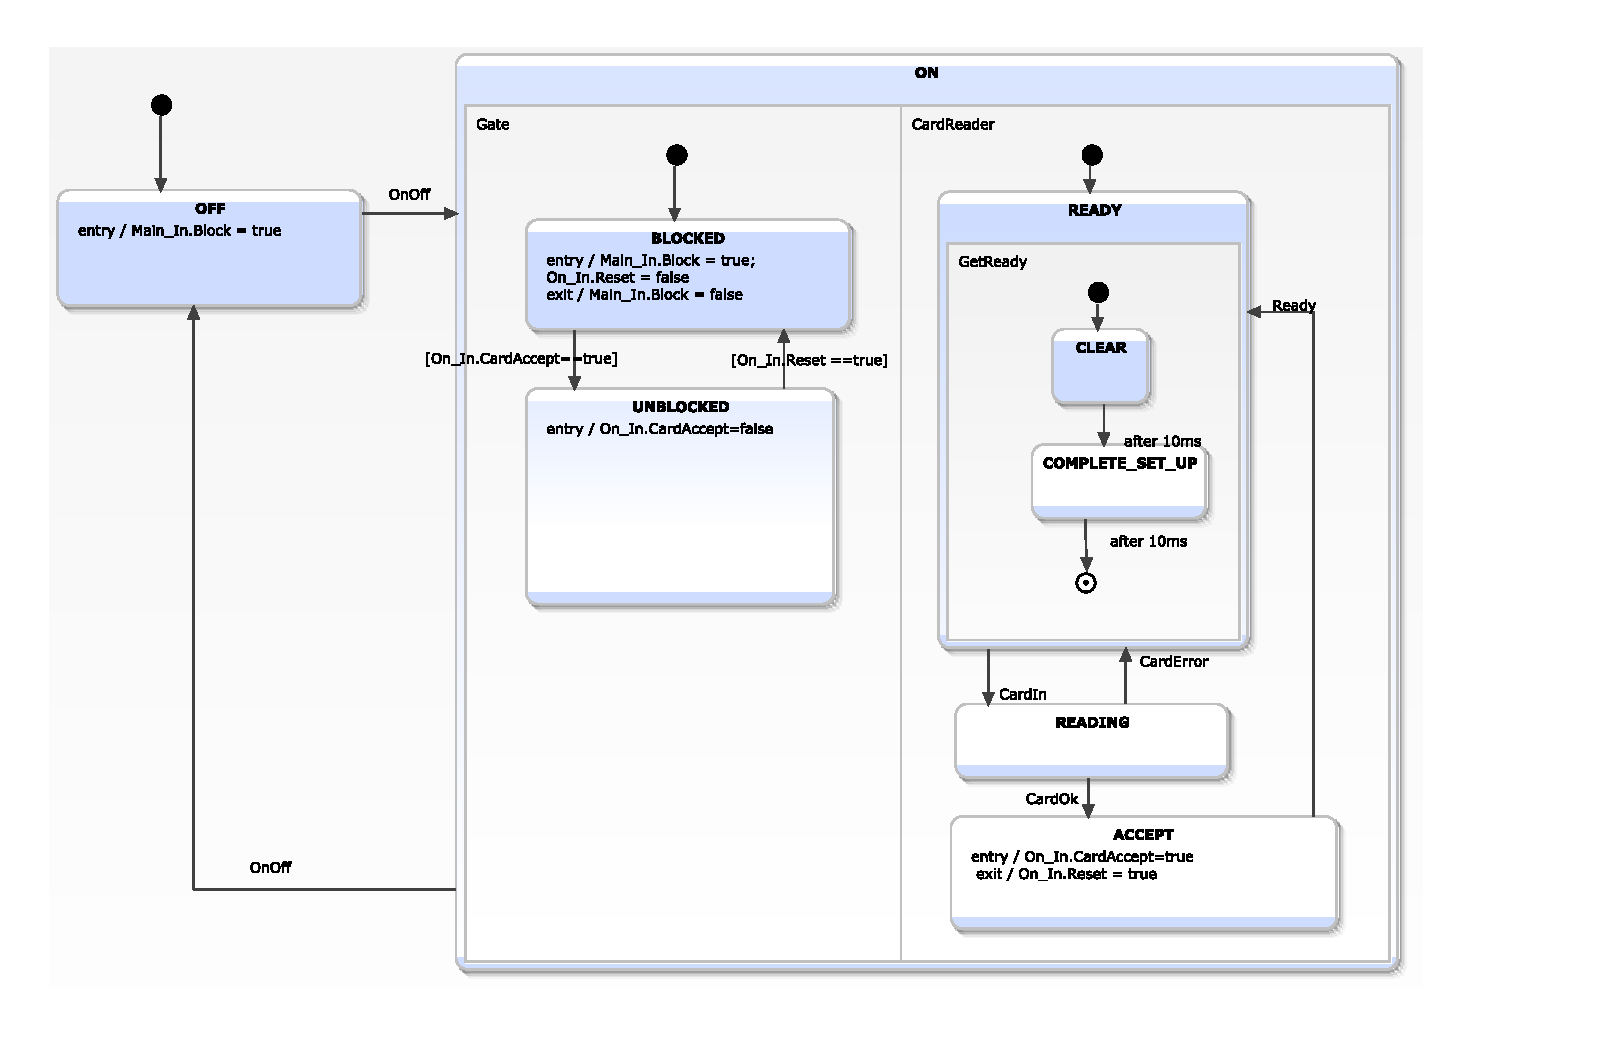
\includegraphics[width=1\textwidth]{caseStudy/TurnstileSimpleModel}
  \caption{SCXML Statechart diagram}
  \label{fig:StatemachineSCXML}
\end{minipage}
\begin{minipage}[]{.5\textwidth}
  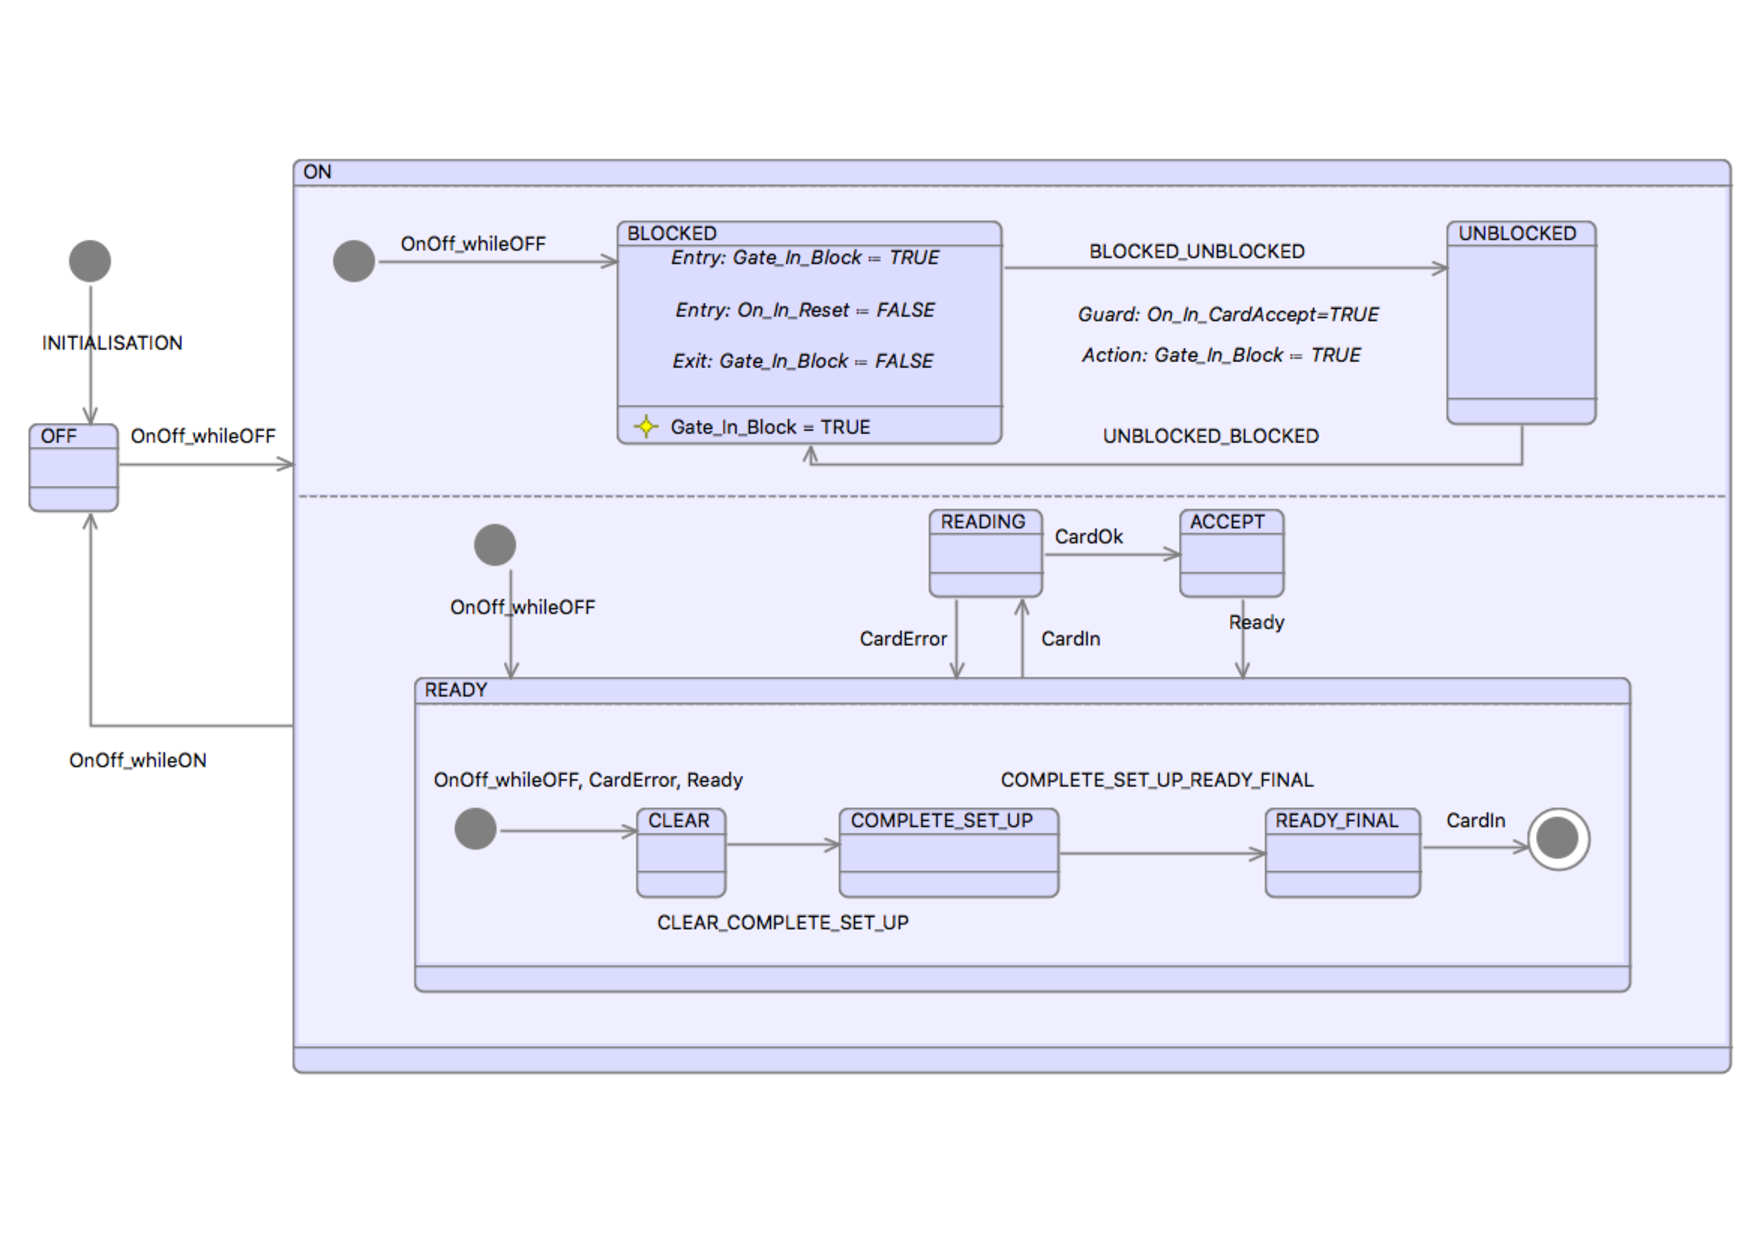
\includegraphics[width=1\textwidth]{caseStudy/TurnstileSimpleModel_iumlb}
  \caption{State-machine diagram in iUML-B at refinement level 3 (partially annotated with guards and actions)}
  \label{fig:StatemachineiUML-B}
\end{minipage}
% \caption{ and }
\end{figure*}

To facilitate Event-B formal verification, extensions to the SCXML 
modelling notation are necessary so that additional modelling features 
required by Event-B can be integrated with the SCXML model.
The SCXML schema allows extension elements and attributes belonging 
to a different namespace to be added. 
The SCXML tooling provides fallback mechanisms so that these extensions are supported 
without the need for syntactic definition. We define a new namespace,  
\emph{iumlb} and add two new elements, \emph{iumlb:invariant} and 
\emph{iumlb:guard} as well as a 
% \emph{iumlb:guard} (Table \ref{iumlb_elements_table}) as well as a 
number of new attributes which are shown in Table \ref{iumlb_attributes_table}.
Invariants are not supported in SCXML but are needed to describe 
verifiable properties of a model. 
SCXML transitions only have a single \emph{cond} attribute whereas we need to introduce conjuncts of a transition
condition at various refinement steps. 
We also need to be able to designate some 
invariants or guards as theorems that can be derived from the preceding conjuncts. 
New attributes are introduced to support the predicate (string) and the 
derived (boolean) theorem property of invariants and guards. The concept 
of refinement is not supported in SCXML. We introduce a new integer valued 
attribute, \emph{iumlb:refinement}, which may be attached to any element of 
either namespace in order to specify the refinement level of that element. 


The example in figure \ref{fig:scxml} shows a state, \emph{BLOCKED}, 
containing a transition that owns an \emph{iumlb:guard}.
The guard reflects the \emph{cond} attribute of the transition 
and is introduced at refinement level 2. 
The state also owns an \emph{iumlb:invariant} with the predicate
 \emph{Gate\_In.Block == TRUE}.



% \begin{table}
% \centering
% \caption{New Elements}
% \label{iumlb_elements_table}
%   \begin{tabular}{|c|c|c|}
%   \hline
%           \multicolumn{1}{c}{Element in iumlb:} \vline
%         & \multicolumn{1}{c}{Meaning} \vline
%         & \multicolumn{1}{c}{Legal Attributes in iumlb:} 
%         \\ \hline 

%     invariant
%         & \begin{tabular}[c]{@{}c@{}} 
%               generates an invariant \\ in Event-B or iUML-B 
%           \end{tabular}     
%         & \begin{tabular}[c]{@{}c@{}}
%               % name, derived, \\ refinement,
%               % predicate, \\ comment
%               name, refinement, \\
%               predicate, derived
%           \end{tabular} 
%         \\ \hline 

%     guard 
%         & \begin{tabular}[c]{@{}c@{}} 
%               generates a guard  \\ in Event-B or iUML-B
%           \end{tabular}    
%         & \begin{tabular}[c]{@{}c@{}}
%               % name, derived, \\ refinement, 
%               % predicate, \\ comment
%               name, refinement, \\
%               predicate, derived
%           \end{tabular} 
%         \\ \hline     
% \end{tabular}%
% \end{table}

\begin{table}
\centering
\caption{SCXML Extension Attributes}
\label{iumlb_attributes_table}
  \begin{tabular}{|c|c|c|}
  \hline
      \multicolumn{1}{c}{Attribute name:} \vline
    & \multicolumn{1}{c}{Meaning} \vline
    & \multicolumn{1}{c}{Allowed Parents} 
   \\ \hline 

    label
        & \begin{tabular}[c]{@{}c@{}} 
              string used as the name of an \\
              Event-B event elaborated by \\
              the generated i-UML-B
          \end{tabular}    
        & \begin{tabular}[c]{@{}c@{}}
              scxml:transition
          \end{tabular} 
   \\ \hline 

    refinement
        & \begin{tabular}[c]{@{}c@{}} 
              non-negative integer representing \\
              the refinement level at which \\
              the parent element should \\
              be introduced
          \end{tabular}    
        & \begin{tabular}[c]{@{}c@{}}
              scxml:scxml, scxml:datamodel, \\ 
              scxml:data, scxml:state, \\
              scxml:parallel, scxml:transition, \\
              scxml:onEntry, scxml:onExit, \\
              scxml:assign, iumlb:invariant, \\
              iumlb:guard
          \end{tabular} 
   \\ \hline 

   %  iumlb:comment
   %      & \begin{tabular}[c]{@{}c@{}} 
   %            string used as a comment \\
   %            on the generated \\
   %            iUML-B element
   %        \end{tabular}    
   %      & \begin{tabular}[c]{@{}c@{}}
   %            iumlb:invariant, iumlb:guard, \\
   %            (could be added to more)
   %        \end{tabular} 
   % \\ \hline 

    type
        & \begin{tabular}[c]{@{}c@{}} 
              string used as the membership \\
              set for the Event-B variable \\
              generated from the parent \\
              data element
          \end{tabular}    
        & \begin{tabular}[c]{@{}c@{}}
              scxml:data
          \end{tabular} 
   \\ \hline 

    name
        & \begin{tabular}[c]{@{}c@{}} 
              string used for the name \\
              or label of a generated \\
              iUML-B element
          \end{tabular}    
        & \begin{tabular}[c]{@{}c@{}}
              iumlb:invariant, iumlb:guard
          \end{tabular} 
   \\ \hline 

    predicate
        & \begin{tabular}[c]{@{}c@{}} 
              string used for the predicate \\
              of a guard or invariant
          \end{tabular}    
        & \begin{tabular}[c]{@{}c@{}}
              iumlb:invariant, iumlb:guard
          \end{tabular} 
   \\ \hline 

   derived
        & \begin{tabular}[c]{@{}c@{}} 
              boolean indicating that \\
              the guard is a theorem \\
              (default to false)
          \end{tabular}    
        & \begin{tabular}[c]{@{}c@{}}
              iumlb:invariant, iumlb:guard
          \end{tabular}       
   \\ \hline 
\end{tabular}%
\end{table}

%------------------------------------------------------------------------------


%------------------------------------------------------------------------------

% !TEX root = main.tex

\section{Translation Tool}

The iUML-B tooling is based on the Eclipse Modelling Framework (EMF). 
It is therefore beneficial to load the SCXML model into EMF so that 
our existing model to model transformation technology can be used to 
define the new SCXML to iUML-B translation. An EMF meta-model for SCXML 
is available from the Sirius \cite{??}
project. It supports SCXML functionality as well as providing generic model
loading facilities for new namespace extensions such as those we 
introduce in \ref{sect:extension}.

Hierarchical nested state charts are translated to similar corresponding 
state-machine structures in iUML-B. There are two alternative styles of 
Event-B representation for iUML-B state-machines.  Currently the state-variables 
style is adopted because it is simpler to translate from the SCXML model. 
However, the alternative state-enumeration style has benefits in user readability 
and may be supported in future. This would  require conventions regarding 
the name of the state-machine  to be adopted and used by the modeller in order 
to construct guards that refer to the current value of the state-machine.
SCXML features, such as initial states, entry/exit actions, and transition 
actions have corresponding similar features in iUML-B and their translation 
is relatively straightforward. Since SCXML `final' states, unlike iUML-B 
final states, are more akin to real states, their translation is less straightforward. 
An iUML-B state, final state and transition from the former to the latter are 
added to the corresponding iUML-B state-machine. The transition elaborates 
all Event-B events that are elaborated by transitions that exit the parent 
iUML-B state. 

\subsection{Refinement Levels}
An \emph{iumlb:refinement} attribute is used to indicate the first refinement 
level at which an element should be introduced in the generated iUML-B/Event-B model. 
In general, elements with no refinement attribute adopt that of their parent.  
However, for \emph{iscxml:state} elements, the refinement level refers to any state 
machines generated from the children nested in that state irrespective of whether 
those children specify a different refinement level. This is because generated 
iUML-B states cannot be added to an existing state-machine in later refinements.
For \emph{iumlb:invariants} the generated invariant is only  generated at the 
specified refinement level, not in  subsequent refinements. This is because Event-B 
invariants are visible through all subsequent refinements.

Note that our approach to refinement in SCXML largely restricts us to superposition 
refinement where entirely new details are introduced at each refinement level.  
It may be possible to support ranges in the refinement attribute enabling a model 
element to be replaced by some other element in a true data refinement. We plan to 
investigate this in future work, although, clearly, several coexisting alternative 
representations of the same concept may be problematic for the SCXML semantics.

\subsection{Constructing event elaborated by transitions}
The Event-B events that are elaborated by an iUML-B  transition are named as follows. 

\begin{enumerate}
\item If the transition has \emph{iumlb:label} attributes, events are generated 
and named according to the label attributes.
\item If the transition's source is an initial state at the outer state chart 
level the transition elaborates the special Event-B INITIALISATION event. 
\item If the transition's source is an initial state of a nested state chart 
the names of all the events that are associated with incoming transitions to 
the parent state are used.
\item If none of the above provide any labels, a default  `source\_target' format is used.
\end{enumerate}

Trigger events are deliberately not used for transition events because we 
want to keep them as a separate concept from transition firing in line 
with SCXML semantics.

\subsection{Data elements}
Data elements, collated in \emph{iscxml:datamodel} elements, model ancillary 
variables in the way usual SCXML style. Data elements are translated to 
Event-B variables of type given in an \emph{iumlb:type} attribute translated 
into an Event-B subset invariant.  The \emph{iscxml:id} attribute of the 
\emph{iscxml:data} element is interpreted as the name of the variable and 
the value is used as the right hand side of an assignment action to initialise 
the variable.  Some syntax conversion is performed to convert the predicate from 
SCXML format into the Event-B mathematical language. The variable is introduced 
at the same refinement level as the parent element that contains it.


%------------------------------------------------------------------------------

%%% Local Variables: 
%%% mode: latex
%%% TeX-master: "HDMachine"
%%% End: 


%------------------------------------------------------------------------------


\section{Case Study}
\label{sect:caseS}

\textcolor{red}{Find a system that we can model and some how describe the benefits 
(e.g. model simplification) of using a specific syntax over the other.
	\begin{itemize}
		\item What model behavior can you capture with each semantic?
		\item What properties of the model are easier to simulate?
		\item Where do we introduce unnecessary complexity?
	\end{itemize}	
}

%------------------------------------------------------------------------------
\section{Conclusion}
\label{sect:concl}

Just to have a reference ~\cite{texniccenter}

%------------------------------------------------------------------------------
\section{Future Work}
\label{sect:future-work}


% \begin{figure}[tb]
%   \begin{centering}
%     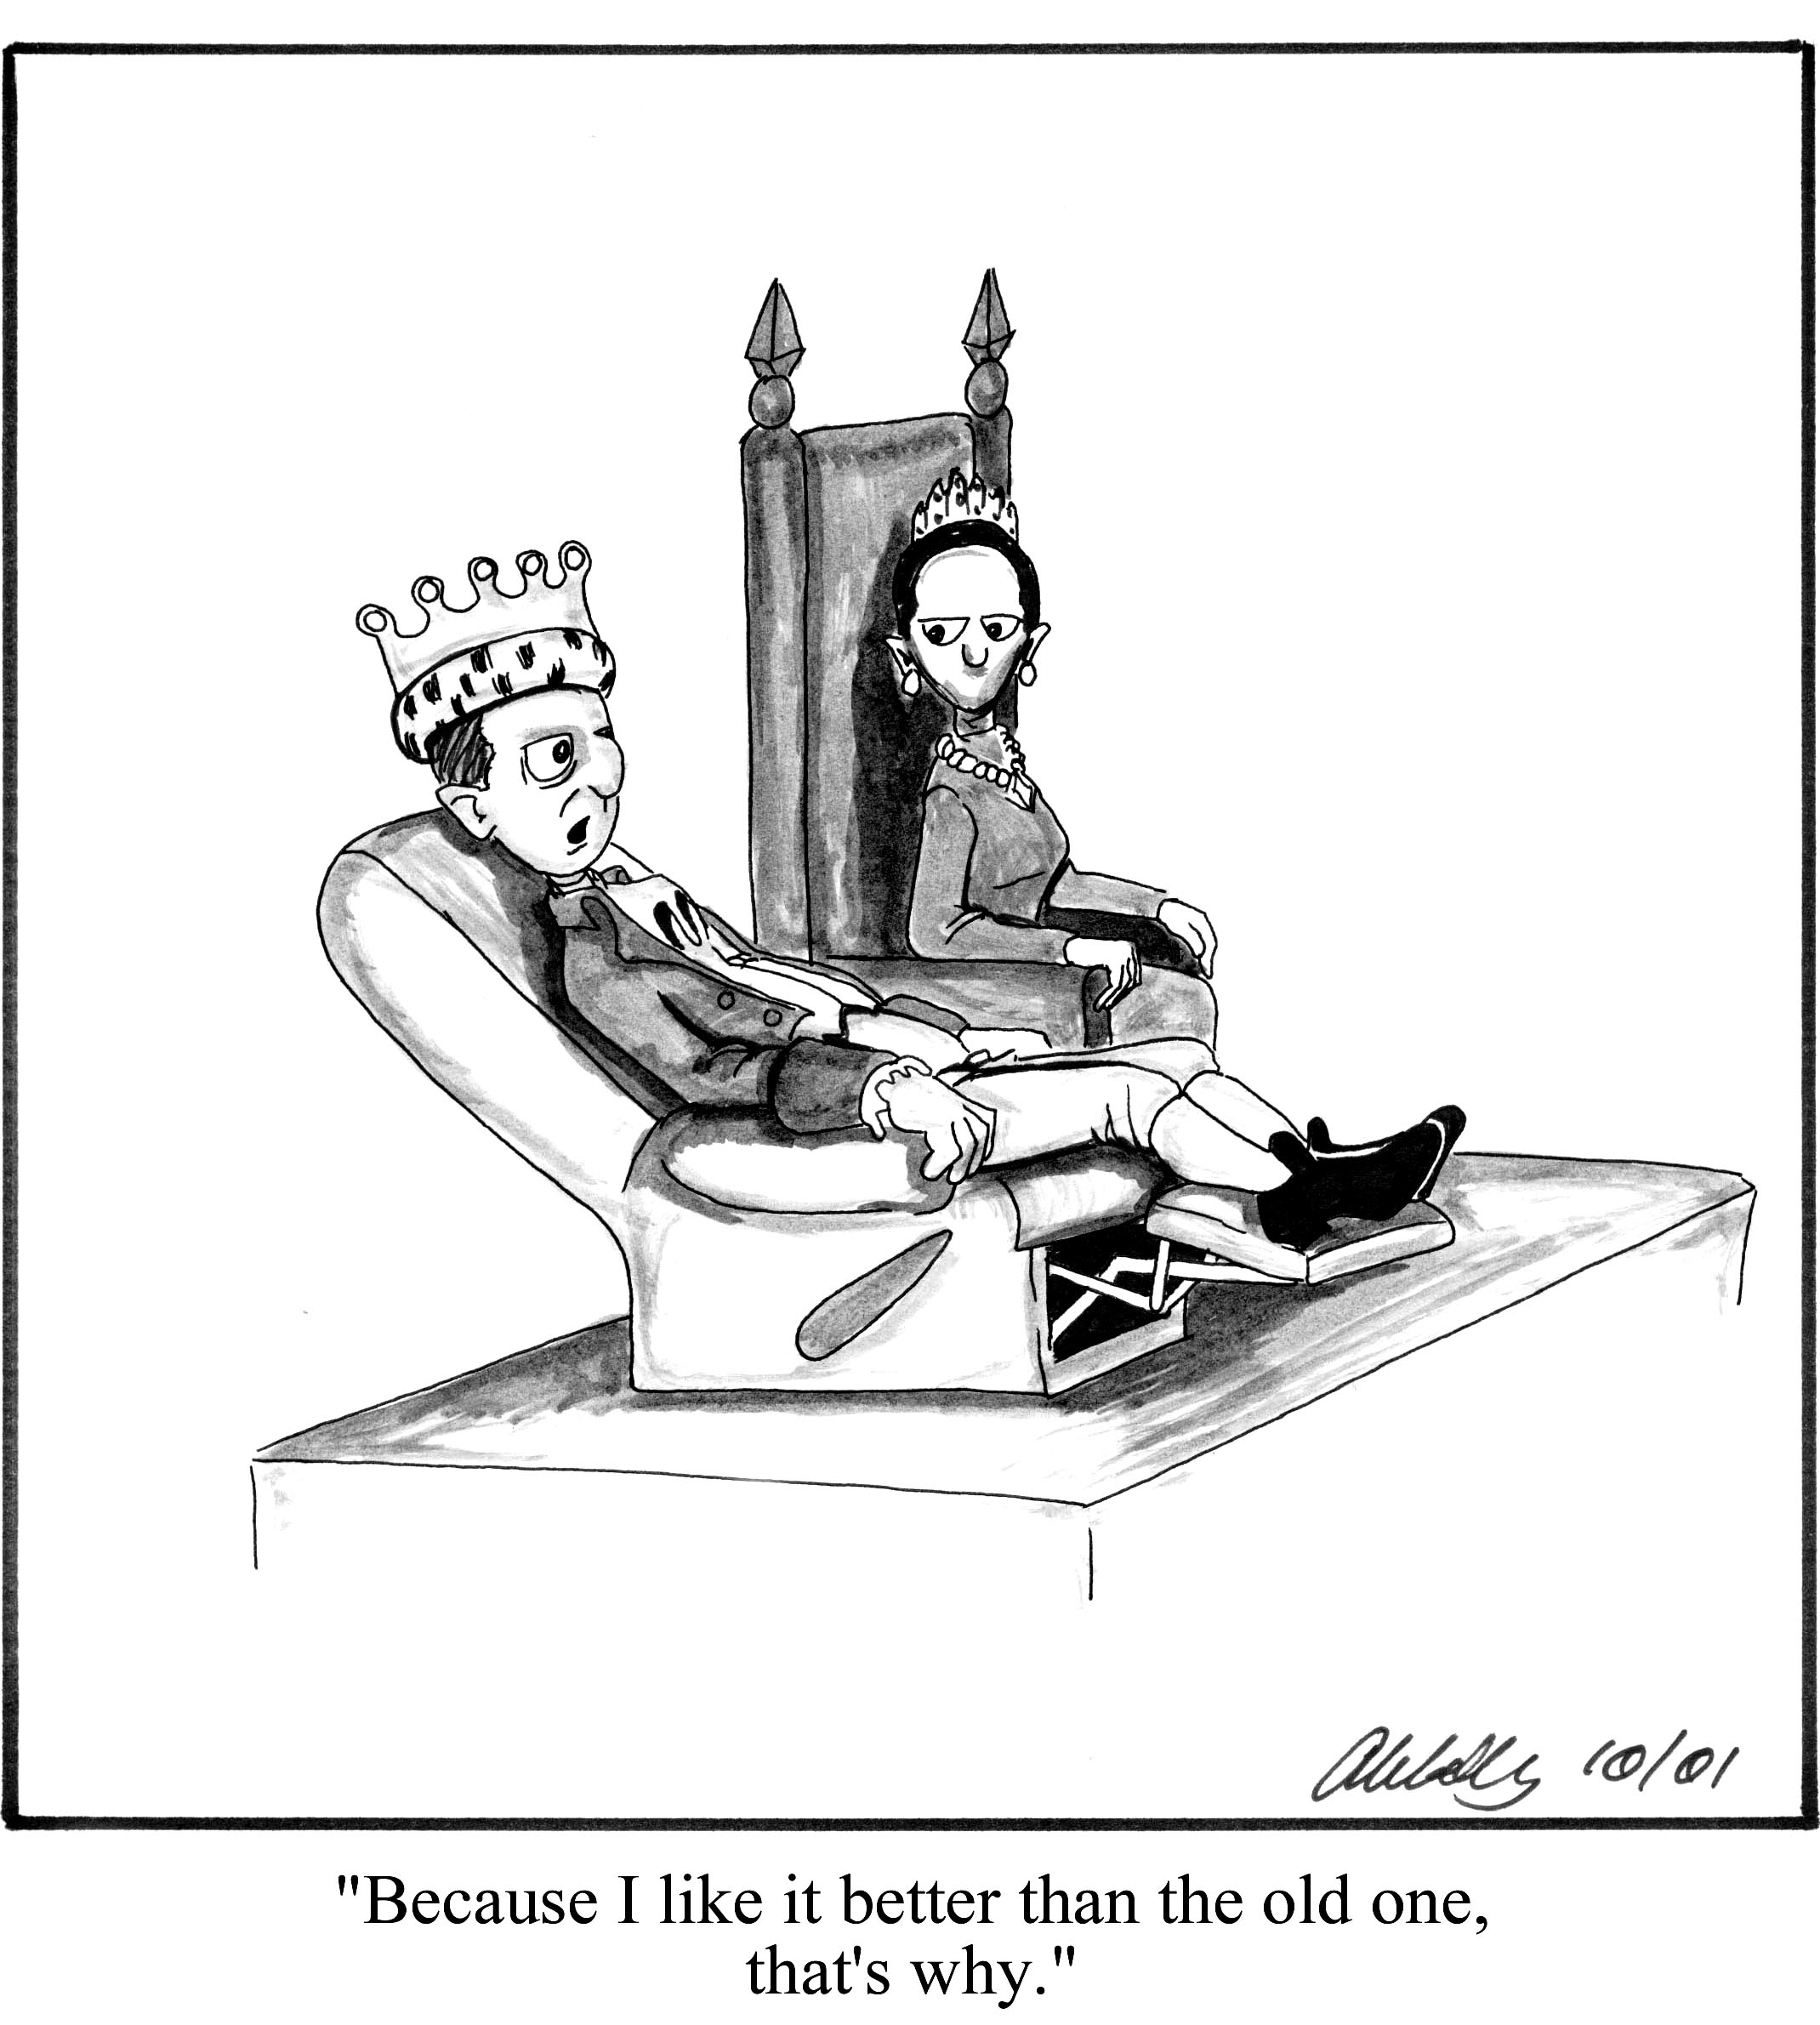
\includegraphics[width=0.5\textwidth]{throneEC.jpg}
%     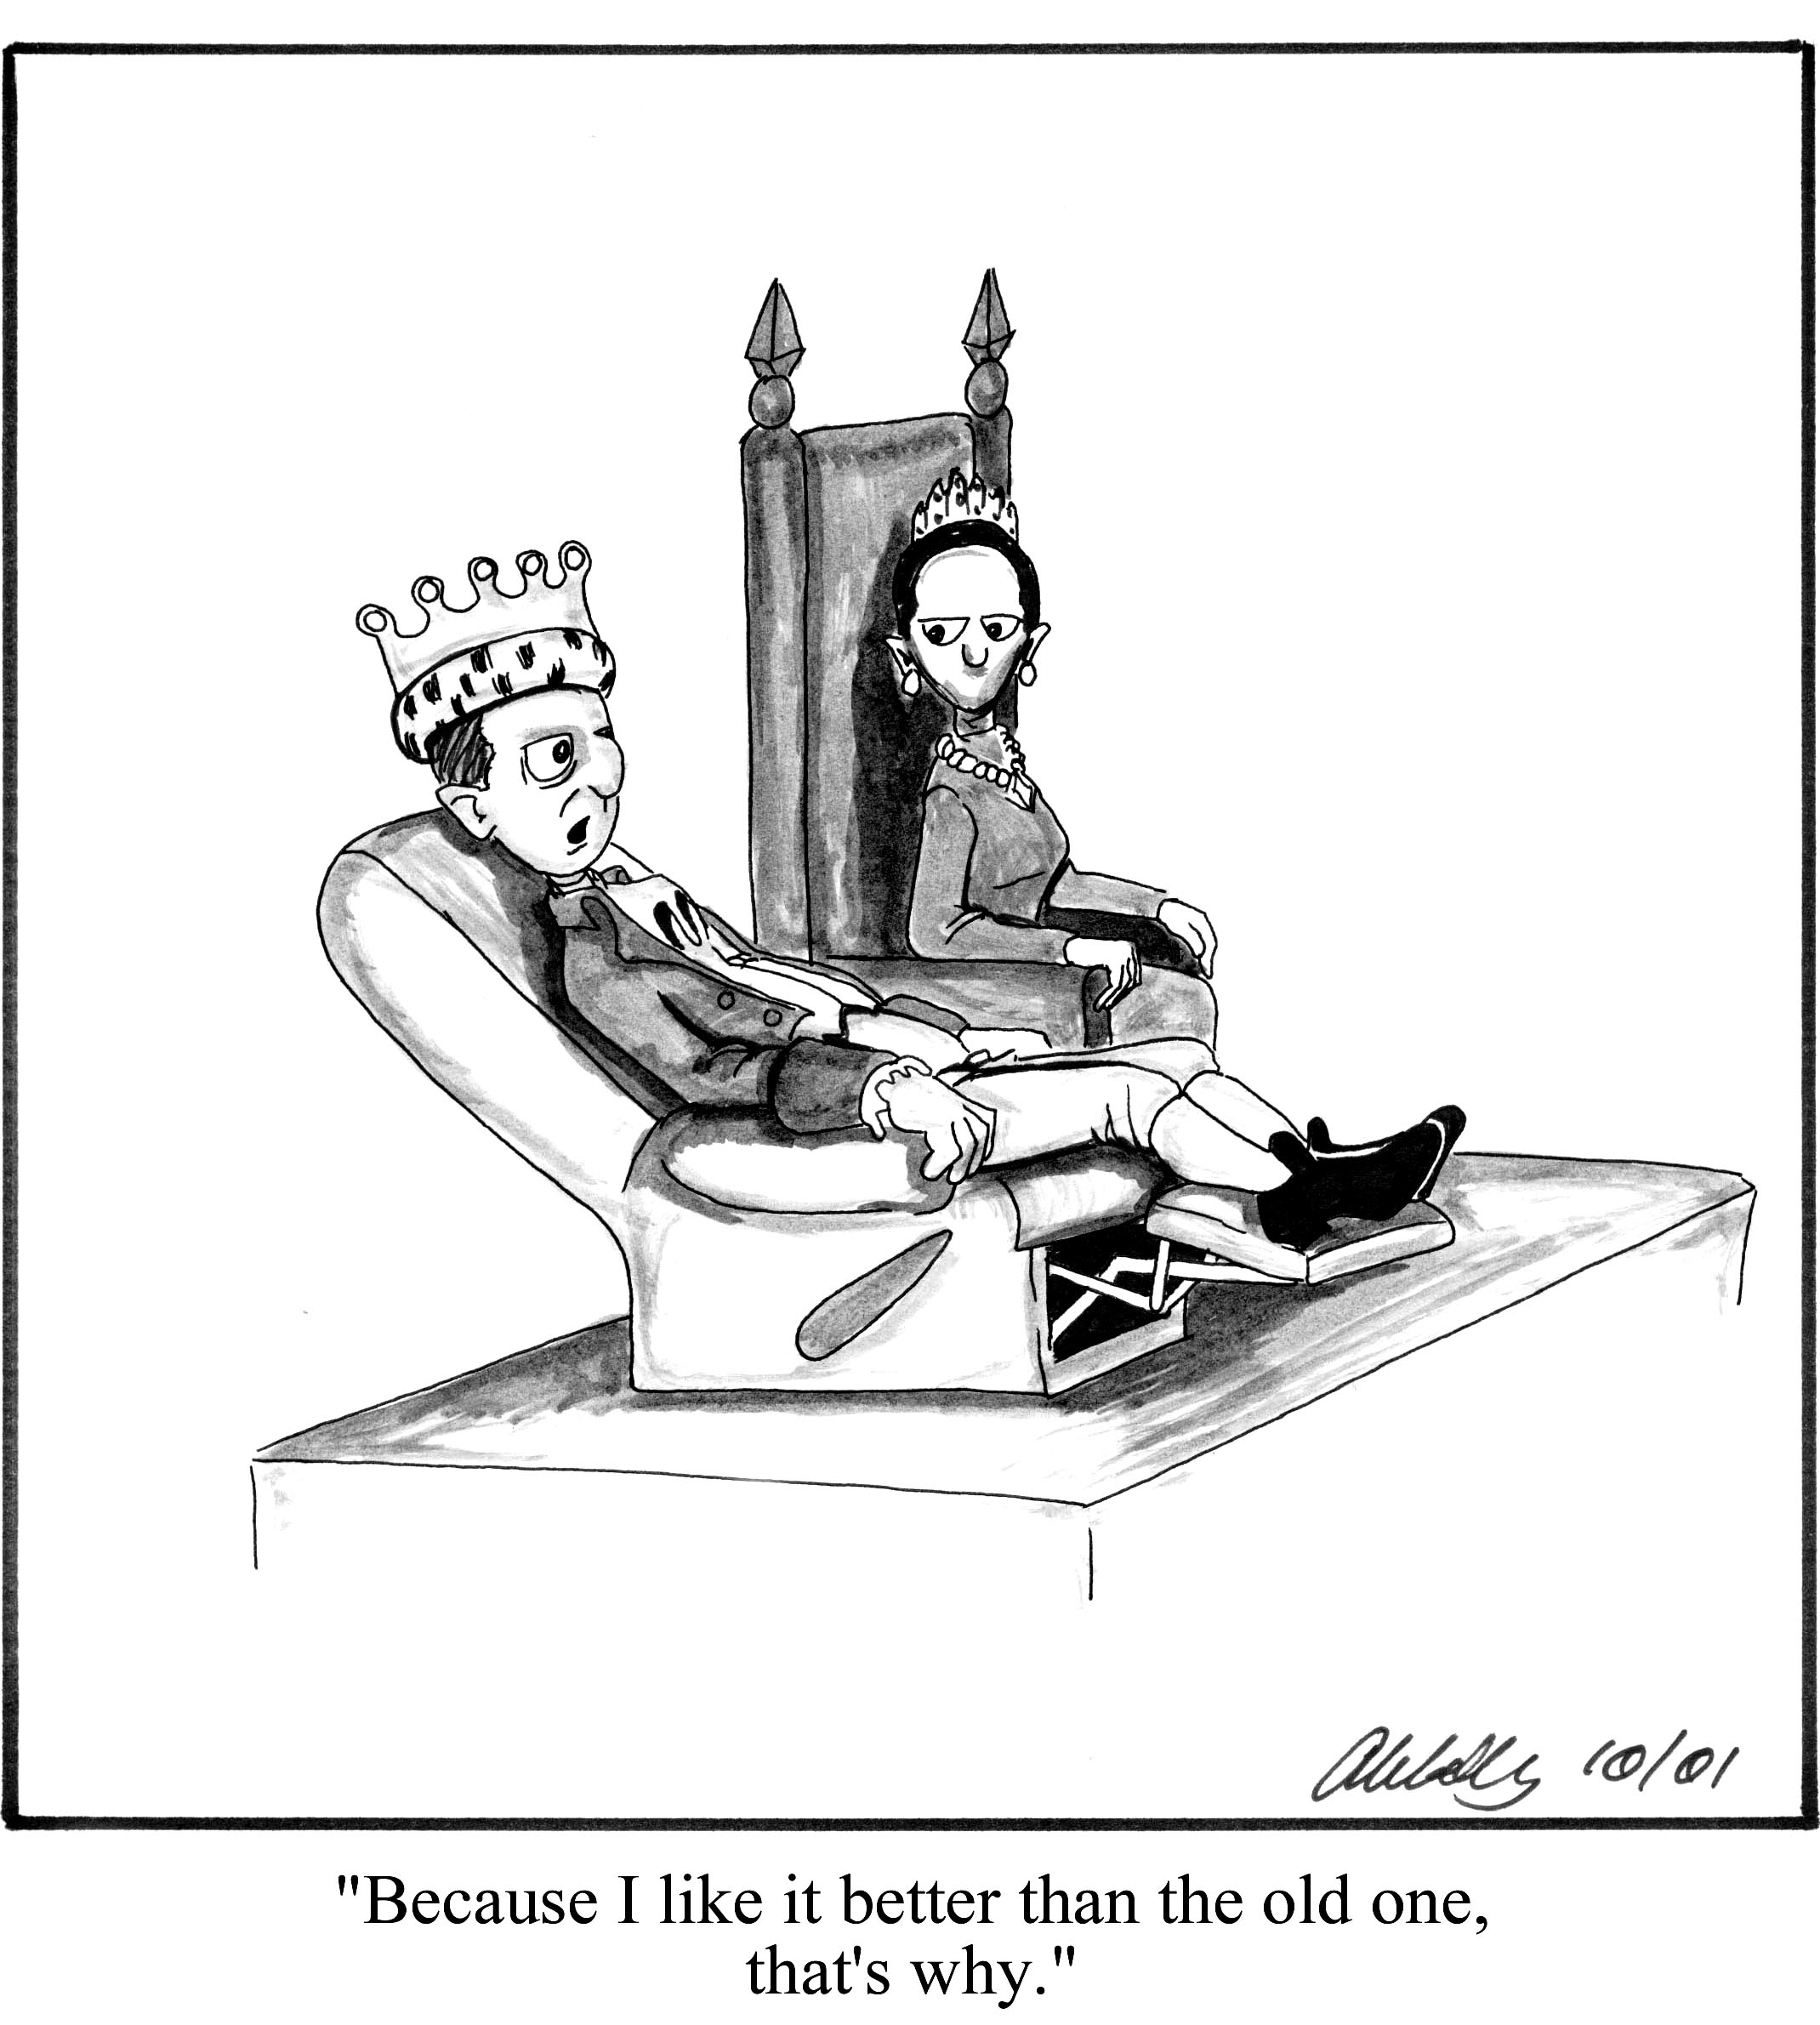
\includegraphics[width=0.3\textwidth]{throneEC.jpg}
%     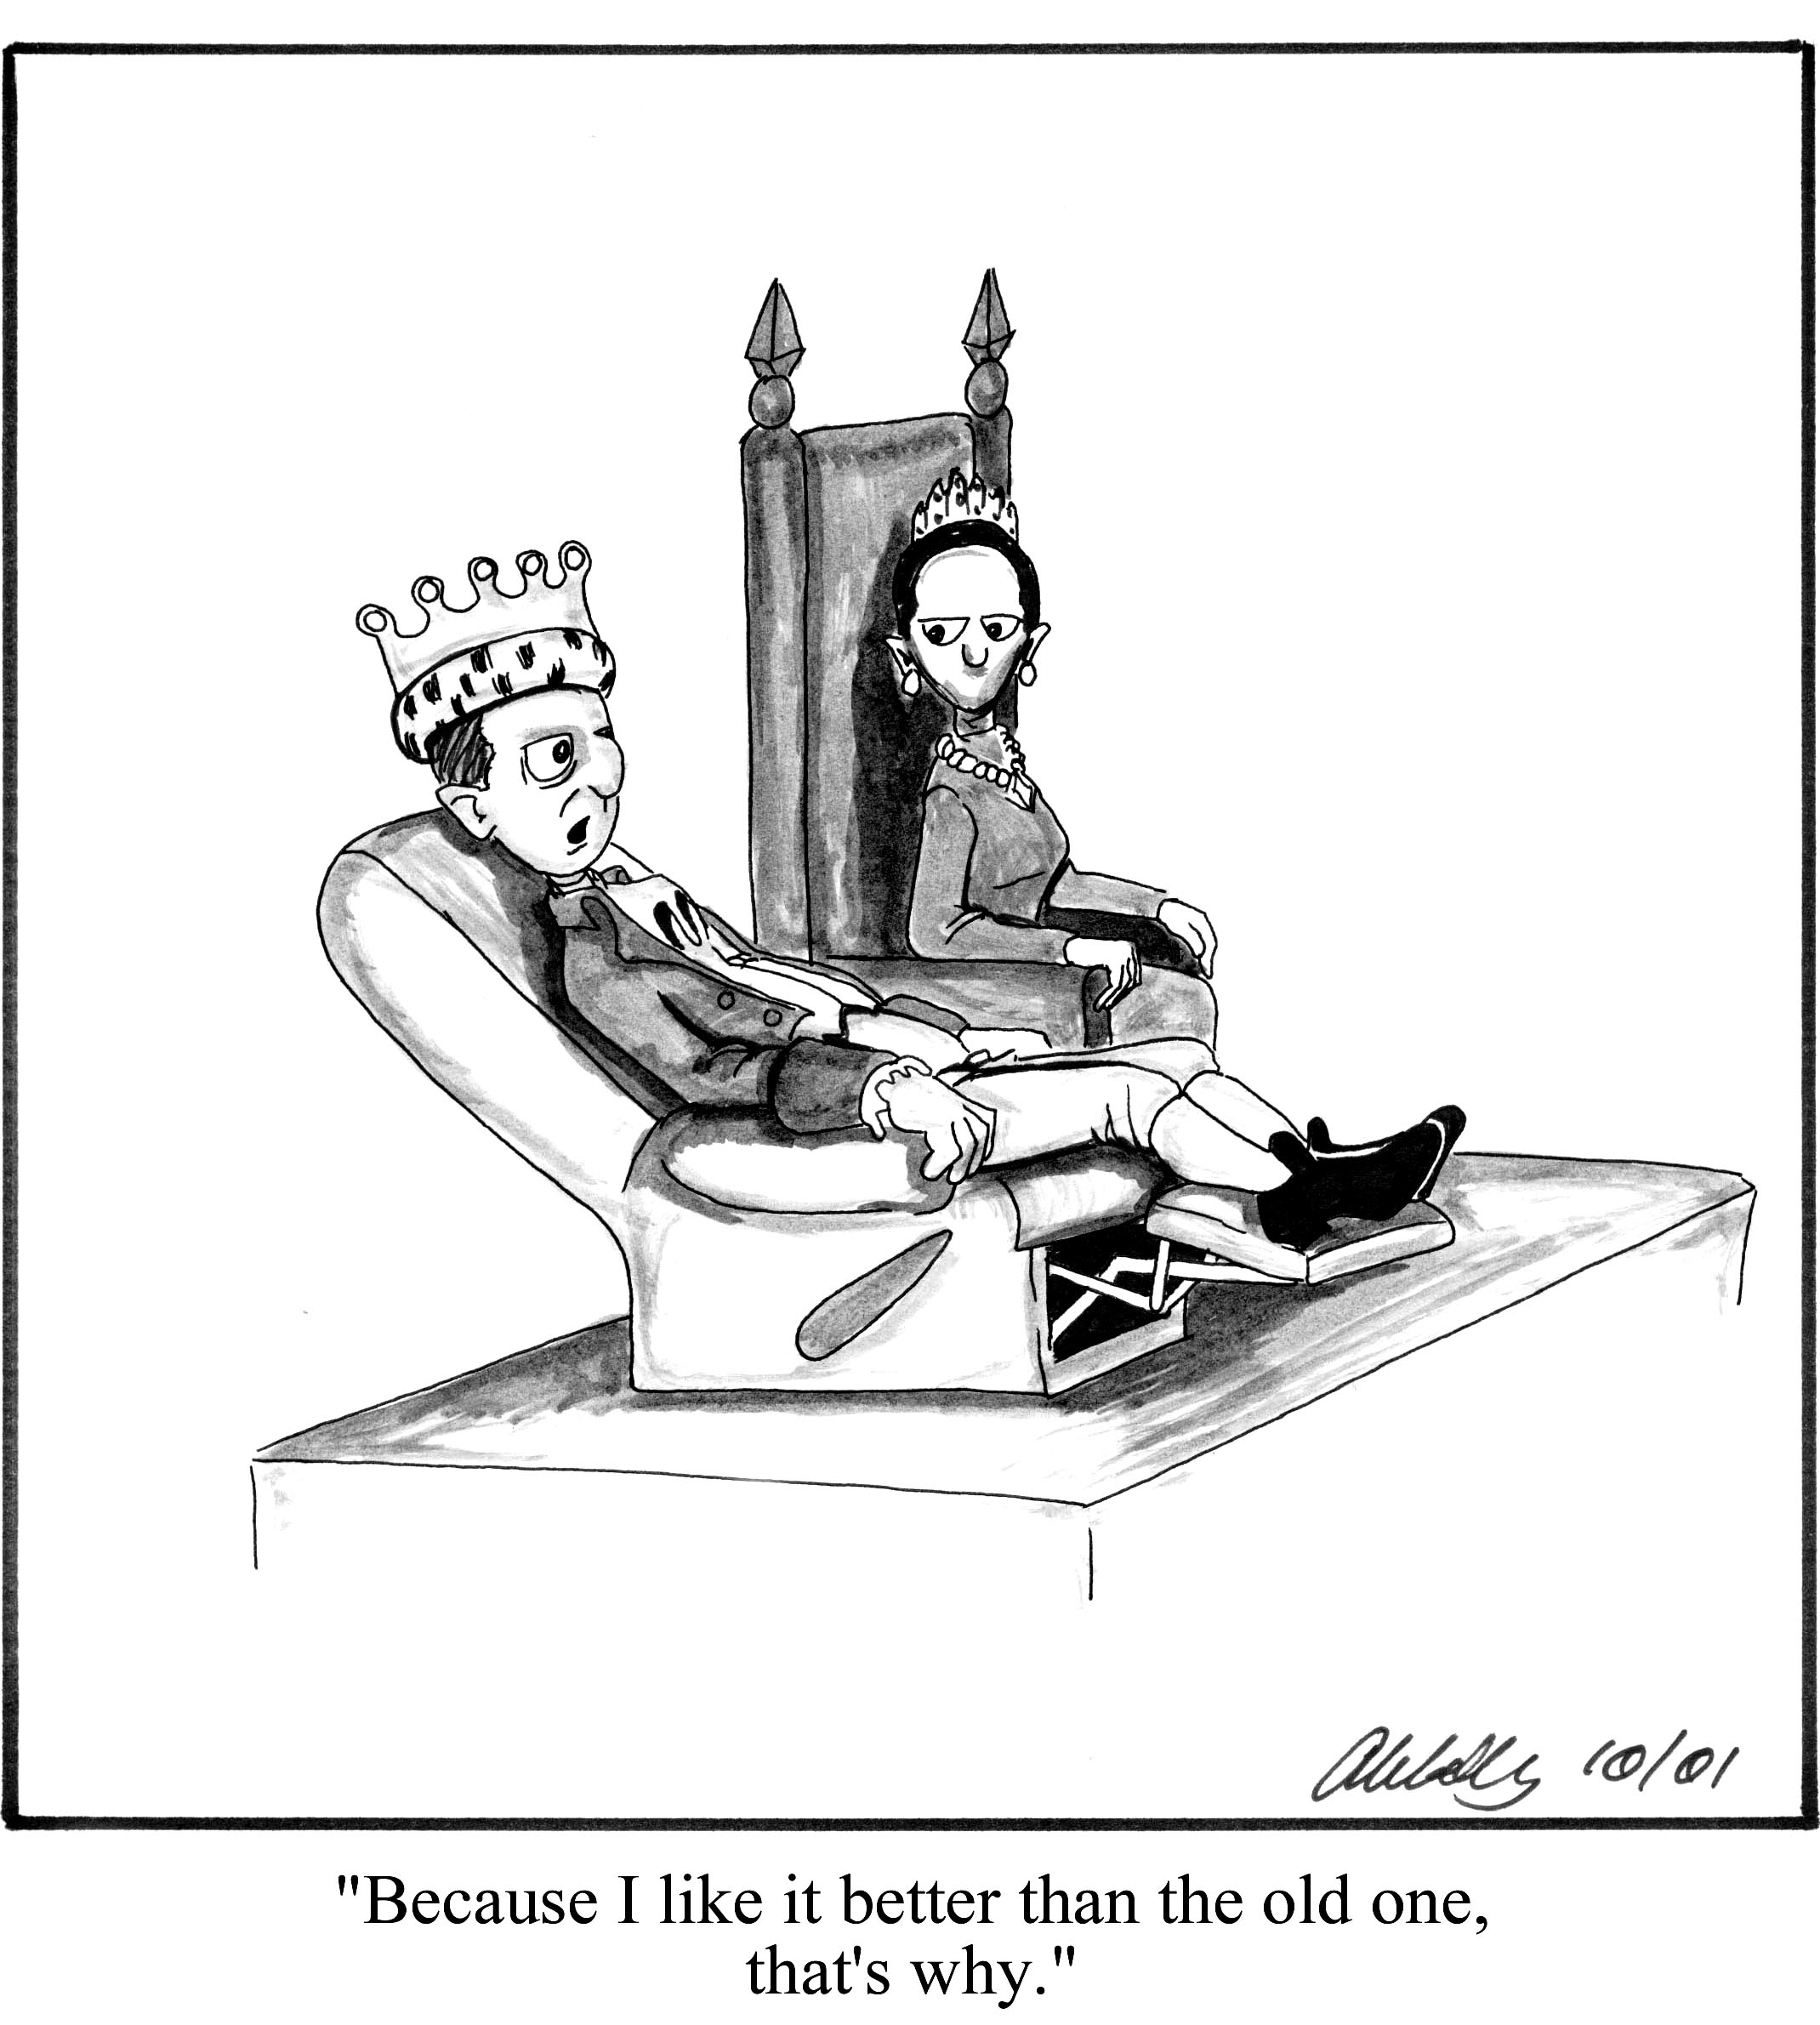
\includegraphics[width=0.15\textwidth]{throneEC.jpg}
%   \end{centering}
%   \caption{Why one should use EasyChair}
%   \label{fig:easythrone}
% \end{figure}

%------------------------------------------------------------------------------
\section{Acknowledgments}
\label{sect:acks}


\label{sect:bib}
\bibliographystyle{plain}
%\bibliographystyle{alpha}
%\bibliographystyle{unsrt}
%\bibliographystyle{abbrv}
\bibliography{easychair}

%------------------------------------------------------------------------------

%------------------------------------------------------------------------------
% Index
%\printindex

%------------------------------------------------------------------------------
\end{document}

